
\documentclass[12pt]{amsart}
\usepackage{geometry} % see geometry.pdf on how to lay out the page. There's lots.
\usepackage{graphicx}	% Including figure files
\usepackage{amsmath}	% Advanced maths commands
\usepackage{amssymb}	% Extra maths symbols
\geometry{a4paper} % or letter or a5paper or ... etc
% \geometry{landscape} % rotated page geometry

% See the ``Article customise'' template for come common customisations

\title{CSE 546 HW1}
\author{David Fleming}
\date{October 14$^{th}$, 2016}

%%% BEGIN DOCUMENT
\begin{document}

\maketitle
\tableofcontents

%%% QUESTION 1 %%%

\section*{Question 1}

\subsection*{1.1}
The expectation value for $max(X_1, X_2)$ is given by
\begin{align}
E[X] = \int max(X_1,X_2) f(x) dx_1 dx_2
\end{align}
where $f(x) = 1$ is the PDF for the uniform random variates.  We consider two regions, one below the line defined by $X = X_1 = X_2$ and one above said line for our integrations.  This gives us the following integral:

\begin{equation} \label{eqn:1.1}
\begin{split}
E[X] & = \int_0^1 \int_{x_2}^1 x_1 dx_1 dx_2 + \int_0^1 \int_{x_1}^1 x_2 dx_2 dx_1 \\
& = \int_0^1 (\frac{1}{2} - \frac{1}{2}x_2^2) dx_2 + \int_0^1 (\frac{1}{2} - \frac{1}{2}x_1^2) dx_1 \\
& = (\frac{1}{2}x_2 - \frac{1}{6}x_2^2) \vert_0^1 + (\frac{1}{2}x_1 - \frac{1}{6}x_1^2) \vert_0^1 \\
& = \frac{2}{3}
\end{split}
\end{equation}

\subsection*{1.2}
Since
\begin{align}
Var[X] = E[X^2] - E[X]^2
\end{align}
and we now know $E[X] = 2/3$, we solve the integral presented above but with the integrand squared as follows
\begin{equation} \label{eqn:1.2}
\begin{split}
E[X^2] & = \int_0^1 \int_{x_2}^1 x_1^2 dx_1 dx_2 + \int_0^1 \int_{x_1}^1 x_2^2 dx_2 dx_1 \\
& = \int_0^1 (\frac{1}{3} - \frac{1}{3}x_2^3) dx_2 + \int_0^1 (\frac{1}{3} - \frac{1}{3}x_1^3) dx_1 \\
& = (\frac{1}{3}x_2 - \frac{1}{12}x_2^4)\vert_0^1 + (\frac{1}{3}x_1 - \frac{1}{12}x_1^4)\vert_0^1 \\
& = \frac{1}{2}
\end{split}
\end{equation}

which when combined with the definition for $Var[X]$ gives
\begin{equation}
Var[X] = \frac{1}{2} - \left( \frac{2}{3} \right)^2 = \frac{1}{18}
\end{equation}

\subsection*{1.3}

Since 
\begin{align}
Cov[X,X_1] = E[X X_1] - E[X]E[X_1]
\end{align}
and we know $E[X]$ from $1.1$ and $E[X_1] = 1/2$ is the trivial result for the uniform distribution from $[0,1]$, we need only calculate the first term as follows:
\begin{equation} \label{eqn:1.3}
\begin{split}
E[XX_1] & = \int_0^1 \int_{x_2}^1 x_1^2 dx_1 dx_2 + \int_0^1 \int_{x_1}^1 x_2 x_1 dx_2 dx_1 \\
& = \int_0^1 (\frac{1}{3} - \frac{1}{3}x_2^3) dx_2 + \int_0^1 x_1(\frac{1}{2} - \frac{1}{2}x_1^2) dx_1 \\
& = (\frac{1}{3}x_2 - \frac{1}{12}x_2^4) \vert_0^1 + (\frac{1}{4}x_1^2 - \frac{1}{8}x_1^4) \vert_0^1 \\
& = \frac{3}{8} 
\end{split}
\end{equation}
giving us
\begin{equation}
Cov[X,X_1] = E[X X_1] - E[X]E[X_1] = \frac{3}{8} - \frac{2}{3}\frac{1}{2} = \frac{1}{24}
\end{equation}

Note: For this question, I collaborated with Matt Wilde.

%%% QUESTION 2 %%%
\section*{Question 2}

\subsection*{2.1}

For the log-likelihood of G given $\lambda$ and i.i.d. samples, we have
\begin{equation} \label{eqn:2.1}
\begin{split}
LL & = \log \left( P(G | \theta)  \right) \\
& = \Pi_i^n P(G_i | \theta) \\
& = \log \left( \frac{\lambda^{\Sigma_i^n k_i} e^{-\lambda n}}{\Pi_i^n k_i !} \right) \\
& = \Sigma_i^n k_i \log \lambda - \lambda n - \log \Pi_i^n k_i !
\end{split}
\end{equation}

\subsection*{2.2}

To compute the MLE for $\lambda$ in general,
\begin{equation} 
\begin{split}
\frac{\partial}{\partial \lambda} \left[ LL \right] = 0
\end{split}
\end{equation}
which yields

\begin{equation} \label{eqn:2.2}
\begin{split}
0 & = \frac{\partial}{\partial \lambda} \left( \Sigma_i^n k_i \log \lambda - \lambda n - \log \Pi_i^n k_i ! \right) \\ 
& = \frac{\Sigma_i^n k_i}{\lambda} - n \\
\hat{\lambda}_{MLE} & = \frac{\Sigma_i^n k_i}{n} \\
\end{split}
\end{equation}

\subsection*{2.3}
For the observed set G, I use Eqn.~\ref{eqn:2.2} to compute $\lambda_{MLE}$ as
\begin{equation}
\hat{\lambda}_{MLE} = \frac{4+1+3+5+5+1+3+8}{8} = 3.75
\end{equation}

Note: For this question, I collaborated with Matt Wilde.

%%% QUESTION 3 %%%

\section*{Question 3}

\subsection*{3.1}

TODO

\subsection*{3.2}

Since in matrix notation we have $\hat{Y} = HY$, I can write 
\begin{equation}
\hat{y_i} = \sum_{j=1}^N H_{ij}y_j
\end{equation}
where $\hat{y}$ has length $N$.

\subsection*{3.3}

To show that $\hat{Y}^{(-i)}$ is the estimator which minimizes SSE for the given $Z_j$, first I substitute $Z_j$ for $y_i$ in the given expression for SSE to get the following
\begin{equation}
SSE = \sum_{j=1}^N (Z_j - \hat{y_j})^2.
\end{equation} 

Now, I expand the above expression for SSE using the definition of $Z_j$

\begin{equation}
\begin{split}
SSE & = \sum_{j \neq i}^N (y_j - \hat{y_j})^2  + (\hat{y}_i^{(-i)} - \hat{y_i})^2
\end{split}
\end{equation}
which reduces to the original SSE with an additional $i = j$ term.  Therefore $\hat{Y}^{(-i)}$ must be the estimator which minimizes the SSE for $Z$.

\subsection*{3.4}

Analogous to the answer to Question 3.2, I can write $\hat{Y}^{(-i)} = HZ$ or in summation notation,
\begin{equation}
\hat{y}_i^{(-i)} = \sum_{j = 1}^N H_{ij}Z_j
\end{equation}

\subsection*{3.5}

To show that $\hat{y}_i - \hat{y}_i^{(-i)} = H_{ii}y_i - H_{ii}\hat{y}_i^{(-i)} $, I will take the left-hand side (LHS) of the equation and expand it with my definitions for $\hat{y}_i $ and $\hat{y}_i^{(-i)}$ from my answers to 3.2 and 3.4 as follows

\begin{equation}
\begin{split}
\hat{y}_i - \hat{y}_i^{(-i)}  & = \\
\sum_{j = 1}^N H_{ij}y_j - \sum_{j = 1}^N H_{ij}Z_j & = \\
\sum_{j \neq i}^N H_{ij}y_j + H_{ii}y_i - \sum_{j \neq i}^N H_{ij}y_j - H_{ii}\hat{y}_i^{(-i)} & = \\
H_{ii}y_i - H_{ii}\hat{y}_i^{(-i)} & = RHS
\end{split}
\end{equation}
as the $j \neq i$ term in $Z_j$ allows us to cancel the summation terms, giving us the RHS as posited.

\subsection*{3.6}

To derive the expected result, first I will rearrange $\hat{y}_i - \hat{y}_i^{(-i)} = H_{ii}y_i - H_{ii}\hat{y}_i^{(-i)}$ as follows
\begin{equation}
\begin{split}
\hat{y}_i - \hat{y}_i^{(-i)} & = H_{ii}y_i - H_{ii}\hat{y}_i^{(-i)}  \\
\hat{y}_i - H_{ii}y_i & =  \hat{y}_i^{(-i)} - H_{ii}\hat{y}_i^{(-i)} \\
\hat{y}_i - H_{ii}y_i & =  (1 - H_{ii})\hat{y}_i^{(-i)} \\
\hat{y}_i^{(-i)} & = (\hat{y}_i - H_{ii}y_i) \frac{1}{1 - H_{ii}}.
\end{split}
\end{equation} 
I now insert this expression for $\hat{y}_i^{(-i)}$ into the expression for LOOCV and reduce to derive the following
\begin{equation}
\begin{split}
LOOVC & = \sum_{i = 1}^N (y_i - \hat{y}_i^{(-i)})^2 \\
& = \sum_{i = 1}^N \left( y_i -  (\hat{y}_i - H_{ii}y_i) \frac{1}{1 - H_{ii}} \right)^2 \\
& = \sum_{i = 1}^N \left( y_i\frac{1 - H_{ii}}{1 - H_{ii}} -  \frac{\hat{y}_i}{1 - H_{ii}}  + \frac{H_{ii}y_i}{1 - H_{ii}}  \right)^2 \\
& = \sum_{i = 1}^N \left( \frac{y_i - \hat{y_i}}{1 - H_{ii}} \right)^2.
\end{split}
\end{equation}

The algorithmic complexity is TODO.

%%% QUESTION 4 %%%

\section*{Question 4}

Note: Both both subquestions 1 and 2, I assume that the too small or too large $\lambda$s bias the model to a too complex or too simple model relative to the optimum model complexity, respectively.

\subsection*{4.1: Too Small a $\lambda$}
\subsubsection*{4.1.a}
For both LASSO and Ridge Regression (RR), the error on the training set would decrease as the penalty term for both regression techniques would be effectively negligible.  With small $\lambda$, the regularization penalty is also small causing both regression techniques to tend towards least squares regression (LSR) and allow for more complex models which overfit the training data and hence leading to smaller training set error.  For example, too small of a $\lambda$ could push both LASSO and RR to favor a high-order polynomial model when the underlying data is linear.

\subsubsection*{4.1.b}
For both LASSO and RR, too small a $\lambda$ leads to overfitting on the training set.  With a model overfit on the training set, it will do a poor job of generalizing to new data and hence will poorly fit the testing set leading to larger testing error.

\subsubsection*{4.1.c}
For both LASSO and RR, too small a $\lambda$ yields too small of a complexity penalty causing both algorithms to tend towards the LSR solution.  In this case, $\hat{\omega}$ could get large via overfitting.  RR, however, will likely predict larger $\hat{\omega}$ than LASSO as RR's $l_2$ norm penalty primarily seeks to control the magnitude of the weight vector, hence biasing towards larger values in this case as the penalty decreases, while LASSO seeks a sparse solution.


\subsubsection*{4.1.d}
With LASSO, too small of a $\lambda$ would yield more non-zero parameters since a smaller regularization penalty will prevent many of the elements of $\hat{\omega}$ from being set to 0 under LASSO's sharp $l_1$ norm penalty which tries to make $\hat{\omega}$ sparse.  For RR, too small of a $\lambda$ would have little effect on the number of non-zero parameters as RR's regularization penalty deals with constraining the magnitude of $\hat{\omega}$ as opposed to forcing it to be sparse.

\subsection*{4.2: Too Large a $\lambda$}
\subsubsection*{4.2.a}
For both regression techniques, too large of a $\lambda$ will yield larger training set error as the regularization penalty will select for simpler models that could poorly fit the data.  For example, too large of a $\lambda$ could push both LASSO and RR to favor a linear model when the underlying data is quadratic.

\subsubsection*{4.2.b}
For both LASSO and RR, too large of a $\lambda$ will yield larger testing set error since the models again will be biased towards lower-than-optimal model complexity and hence will likely yield a poor fit to future data similar to why the error on the training set is also larger in this case.

\subsubsection*{4.2.c}
For both LASSO and RR, too large of a $\lambda$ will yield smaller $\hat{\omega}$ as the larger regularization penalty restricts the weight vector.  RR, however, will likely predict smaller $\hat{\omega}$ than LASSO as RR's $l_2$ norm penalty primarily seeks to control the magnitude of the weight vector, hence biasing towards smaller values in this case, while LASSO seeks a sparse solution.

\subsubsection*{4.2.d}
For LASSO, a larger $\lambda$ will yield a sparser solution via its $l_1$ norm regularization penalty and hence will have fewer nonzero elements in $\hat{\omega}$ than RR.  In the large $\lambda$ limit, RR will also yield fewer nonzero elements in $\hat{\omega}$ only because its large regularization penalty makes coefficients in its weight vector small and hence potentially pushing some towards 0.

Note: For this question, I collaborated with Matt Wilde.

%%% QUESTION 5 %%%

\section*{Question 5}
TODO

%%% QUESTION 6 %%%

\section*{Question 6}

Note: The following scripts (attached) include all code used to solve this question: {\tt hw1$\_$6.py, mnist$\_$utils.py, regression$\_$utils.py, ridge$\_$utils.py}.

Here, the I build a linear classifier by minimizing the following Ridge Regression Loss:
\begin{equation} \label{eqn:RR_loss}
\text{min}_{\omega} = \frac{1}{N} \Sigma_{i = 1}^N (y_i - \omega \cdot x_i)^2 + \lambda || \omega ||^2.
\end{equation}
In general, the RR regression weight vector can be solved for analytically via the following
\begin{equation} \label{eqn:RR_w}
\hat{\omega_{ridge}} = (\lambda I_D + X^T X)^{-1} X^T y
\end{equation}
however the matrix inversion required is not only computationally expensive but also can be numerically unstable.  Instead, I minimize Equation~\ref{eqn:RR_loss} by following the formulae in the textbook (see Murphy Section 7.5.2) which involves centering the data and augmenting X with the Cholesky decomposition of the precision matrix and y with a vector of 0s.  This yields the MAP estimate
\begin{equation} \label{eqn:RR_w_murphy}
\hat{\omega_{ridge}} = (\tilde{X}^T \tilde{X})^{-1} \tilde{X}^T \tilde{y}.
\end{equation}

\subsection*{6.1}
I adopt a regularization constant $\lambda = 1$.  For the purpose of classification, I label a digit as 2 if $\omega \cdot x > c$.  To compute the threshold $c$, I first take the training labels and set all instances of 2 to 1 and all other digits to 0.  Then, I mask the training labels to get a vector that encodes which rows of the training data yield a 2.  Next, I fit the training set with my ridge regression model via Equation~\ref{eqn:RR_w_murphy} and compute my predictions over the training set $\hat{y} = \omega_0 + X_{train}\hat{\omega}$.  Then, using my previously computed mask, I find the entries of my predictions $\hat{y}$ that should be labeled as 2s according to the true training labels.  I take the median of these values to find an approximate threshold $c = 0.589$.  When I apply this model to the testing set, and predicted value with $\omega \cdot x > c$ will be set to 1 and 0 otherwise.

After training my model, I find a 0/1 and a square loss of 3059 on the training set.  These values are the same because my predictions are either 0 or 1 and the true labels are either 0 or 1.  Note that this loss does not seem terribly high for my heuristic classifier given that there are of order 6,000 2's in the MNIST training set.  However, even a naive classifier that says everything is not a 2 would be correct roughly $90\%$ of the time, therefore I expect my model that does a simple prediction with a poor linear Ridge Regression to do slightly better.

\subsection*{6.2}
On the testing set, I evaluated my model from fitting the training set and apply it to the testing input images to find a 0/1 and a square loss of 545.  Note that it appears that my error on the testing set is actually less than that of the training set!  This, however, is not the case since the training set contains 60,000 samples while the testing set contains 10,000.  If the size of the set over which the model is evaluated is taken into account, my model performs worse on the testing set and hence the testing error is larger as is expected for classifying with a linear regression model.

\subsection*{6.3}
Linear regression is a poor idea for classification since the slope of the predicted line decides which input vector is labeled a 0 and which is labeled a 1.  Instead of ascribing a probability to each estimate, it instead checks to see if it's above or below a given threshold.  This model does not successfully generalize to new data at all since new data points since the slope of the classifying line is so dependent on the training data and new points could dramatically shift the slope of that line, changing which class a given point belongs to.

\subsection*{6.4}
TODO

Note: For this question, I collaborated with Matt Wilde.

%%% QUESTION 7 %%%

\section*{Question 7}

\subsection*{7.1}

\subsubsection*{7.1.1}
If we define
\begin{equation}
\hat{y_i} = X_i \omega + w_0,
\end{equation}
we can rearrange that to get 
\begin{equation}
X_i \omega = \hat{y_i} - w_0.
\end{equation}
Combining that expression with the update rule for $w_0$ from Algorithm 1, we find
\begin{equation}
w_0^{(t+1)} = \sum_{i = 1}^N (y_i - \hat{y_i}^{(t)})/N + w_0^{(t)}
\end{equation}
by substituting out the $X_i \omega$ term in favor of the expression with $\hat{y_i} - w_0$ since $X_i \omega = \sum_j \omega_j X_{ij}$.

Similarly for the new $c_k$ update rule, we can insert
\begin{equation}
w_0 = \hat{y_i} - X_i \omega.
\end{equation}
into the following expression for $c_k$
\begin{equation}
c_k = 2 \sum_{i=1}^N X_{ik}(y_i - (w_0 + \sum_{j \neq k}\omega_j X_{ij}))
\end{equation}
where 
\begin{equation}
-\sum_j X_{ij}\omega_j + \sum_{j \neq k}\omega_j X_{ij} = -X_{ik}\omega_k
\end{equation}
allows us to simplify the expression into 
\begin{equation}
c_k = 2 \sum_{i=1}^N X_{ik}(y_i - \hat{y_i} + X_{ik}\omega_k).
\end{equation}
This final expression no longer includes the summation over $j$.

\subsubsection*{7.1.2}
The dot product of a sparse matrix and a vector takes time proportional to the number of nonzero entries in said sparse matrix.  Therefore if $||X||_0$ is the number of nonzero entries in X, the time complexity to compute $\hat{y} = X\omega + w_0$ is $\mathcal{O}(||X||_0 + N)$.

\subsubsection*{7.1.3}

If $\hat{y}$ is not already computed, it takes $\mathcal{O}(N ||X||_0)$ to compute $\hat{y}$ then $\mathcal{O}(N)$ to loop over all entries of $y$ and $\hat{y}$ to compute $w_0$ yielding a total complexity $\mathcal{O}(N + N||X||_0)$ since we still need only to compute $\hat{y}$ once.  If $\hat{y}$ has already been computed, the time complexity is only $\mathcal{O}(N)$. 

\subsubsection*{7.1.4}

Define $z_j$ to be the number of nonzero elements in the $j-th$ column of X.  If $\hat{y}$ is already computed, the time complexity to compute $\hat{\omega}$ is $\mathcal{O}(N)$ as one needs to loop over N elements while computing both $a_k$ and $c_k$ while computing $w_k$.

\subsubsection*{7.1.5}

I can rearrange the expression for $\hat{y}_i^{(t)}$ to get the following
\begin{equation}
X_i \omega^{(t)} = \hat{y}_i^{(t)} - w_0^{(t)}.
\end{equation}
I insert the above expression for $X_i \omega^{(t)}$ into the equation for $\hat{y}_i^{(t+1)}$ to find the corresponding update rule for the new prediction
\begin{equation}
\hat{y}_i^{(t+1)} = \hat{y}_i^{(t)} + w_0^{(t+1)} - w_0^{(t)}
\end{equation}
where $w_0^{(t+1)}$ was found via the update rule derived in Question 7.1.1 and $w_0^{(t)}$ was the value of $w_0$ at the start of the current iteration.  

If $\hat{y}^{(t)}$ is already computed, the complexity to calculate $\hat{y}^{(t+1)}$ is simply $\mathcal{O}(N)$ as one must loop over the N elements of $\hat{y}^{(t+1)}$ for the computation.

\subsubsection*{7.1.6}

First, define
\begin{equation}
\hat{y}_i^{(t+1)} = \sum_{j \neq k} \omega_j^{(t)}X_{ij} + \omega_k^{(t+1)}X_{ik} + w_0^{(t)}
\end{equation}
to be the new prediction after updating.
Again, I note that 
\begin{equation}
X_i \omega^{(t)} = \hat{y}_i^{(t)} - w_0^{(t)}
\end{equation}
which we can insert that into the above new prediction since $\sum_{j} \omega_j^{(t)}X_{ij} = X_i \omega^{(t)} $ to get 
\begin{equation}
\hat{y}_i^{(t+1)} = \hat{y_i}^{(t)} - w_0^{(t)} - \omega_k^{(t)}X_{ik} + \omega_k^{(t+1)}X_{ik} + w_0^{(t)}
\end{equation}
to be the new prediction after updating.  This expression reduces to the new update rule for $\hat{y}_i^{(t+1)}$ in terms of $\hat{y}_i^{(t)}$
\begin{equation}
\hat{y}_i^{(t+1)} = \hat{y_i}^{(t)} + X_{ik}(\omega_k^{(t+1)} - \omega_k^{(t)}).
\end{equation}

If $\hat{y}_i^{(t)}$ is already computed, the time complexity required to compute $\hat{y}_i^{(t+1)}$ is $\mathcal{O}(N)$ as one must loop over all $N$ elements in $\hat{y}_i^{(t+1)}$.

\subsubsection*{7.1.7}

Combining all the rules derived in 7.1.1 - 7.1.6, we have the Efficient Coordinate Descent Algorithm for LASSO regression.  To estimate the per iteration complexity of the algorithm, we note that within the while loop there are two regimes to consider: within the for loop over all $d$ features and outside said loop.  Outside the loop, the first calculation of $\hat{y}$ is $\mathcal{O}(||X||_0 + N)$ as shown in 7.1.2.  The update rules for $w_0$ and the second update of $\hat{y}$ both take $\mathcal{O}(N)$ yielding a net $\mathcal{O}(||X||_0 + N)$ for the operations outside of the for loop.  Within the for loop over all $d$ features, each operations is $\mathcal{O}(N)$ (see 7.1.1, 7.1.6) as each operation involves looping over $N$ elements to perform simple arithmetic operations.  Since for each loop iteration operations with complexity $\mathcal{O}(N)$ occur, these all occur $d$ times over the course of the loop yielding a net for loop complexity of $\mathcal{O}(Nd)$.  This complexity then combines with the outside of the loop complexity to yield a per iteration complexity of $\mathcal{O}(Nd + ||X||_0 + N)$.  When we only consider the highest power term, this gives a per iteration complexity of the algorithm of $\mathcal{O}(Nd)$.

\subsection*{7.2}

My {\tt python} implementations of both Algorithm 1 and Algorithm 2 are in the attached file {\tt lasso$\_$utils.py} and are named {\tt fit$\_$lasso and fit$\_$lasso$\_$fast}, respectively.  Each function includes the offset term $w_0$ that is not regularized, have the option to take initial conditions for both $\omega$ and $w_0$ and can handle dense or sparse $X$ using the {\tt scipy.sparse} package.

\subsection*{7.3}

\subsubsection*{7.3.1}

In the file {\tt regression$\_$utils.py}, the function {\tt generate$\_$norm$\_$data} generates the synthetic data set according to the procedure outlines in Question 7.3.  To optimize over $\lambda$, I ran a regularization path starting at $\lambda_{max} = 5000$.  This value of  $\lambda_{max}$ was a factor of 3 or so larger than $\lambda_{max} = 2 ||X^{T}(y - \bar{y}) ||_{\infty}$ in order to demonstrate that too large of a regularization penalty yields a null weight vector.  For each iteration, I decreased $\lambda$ by a factor of 2 and initialized my LASSO algorithm with the results of the previous iteration.  For the first iteration, I assumed that $\omega$ was null.  For each iteration, I compared the sparsity pattern of my solution $\hat{w}$ to the true value I generated, $\omega_{true}$ by recording the precision and recall. The results of this regularization path for data generated with $\sigma = 1$ and for data with $\sigma = 10$ is shown in Fig.~\ref{fig:synth_reg}.

\begin{figure}
	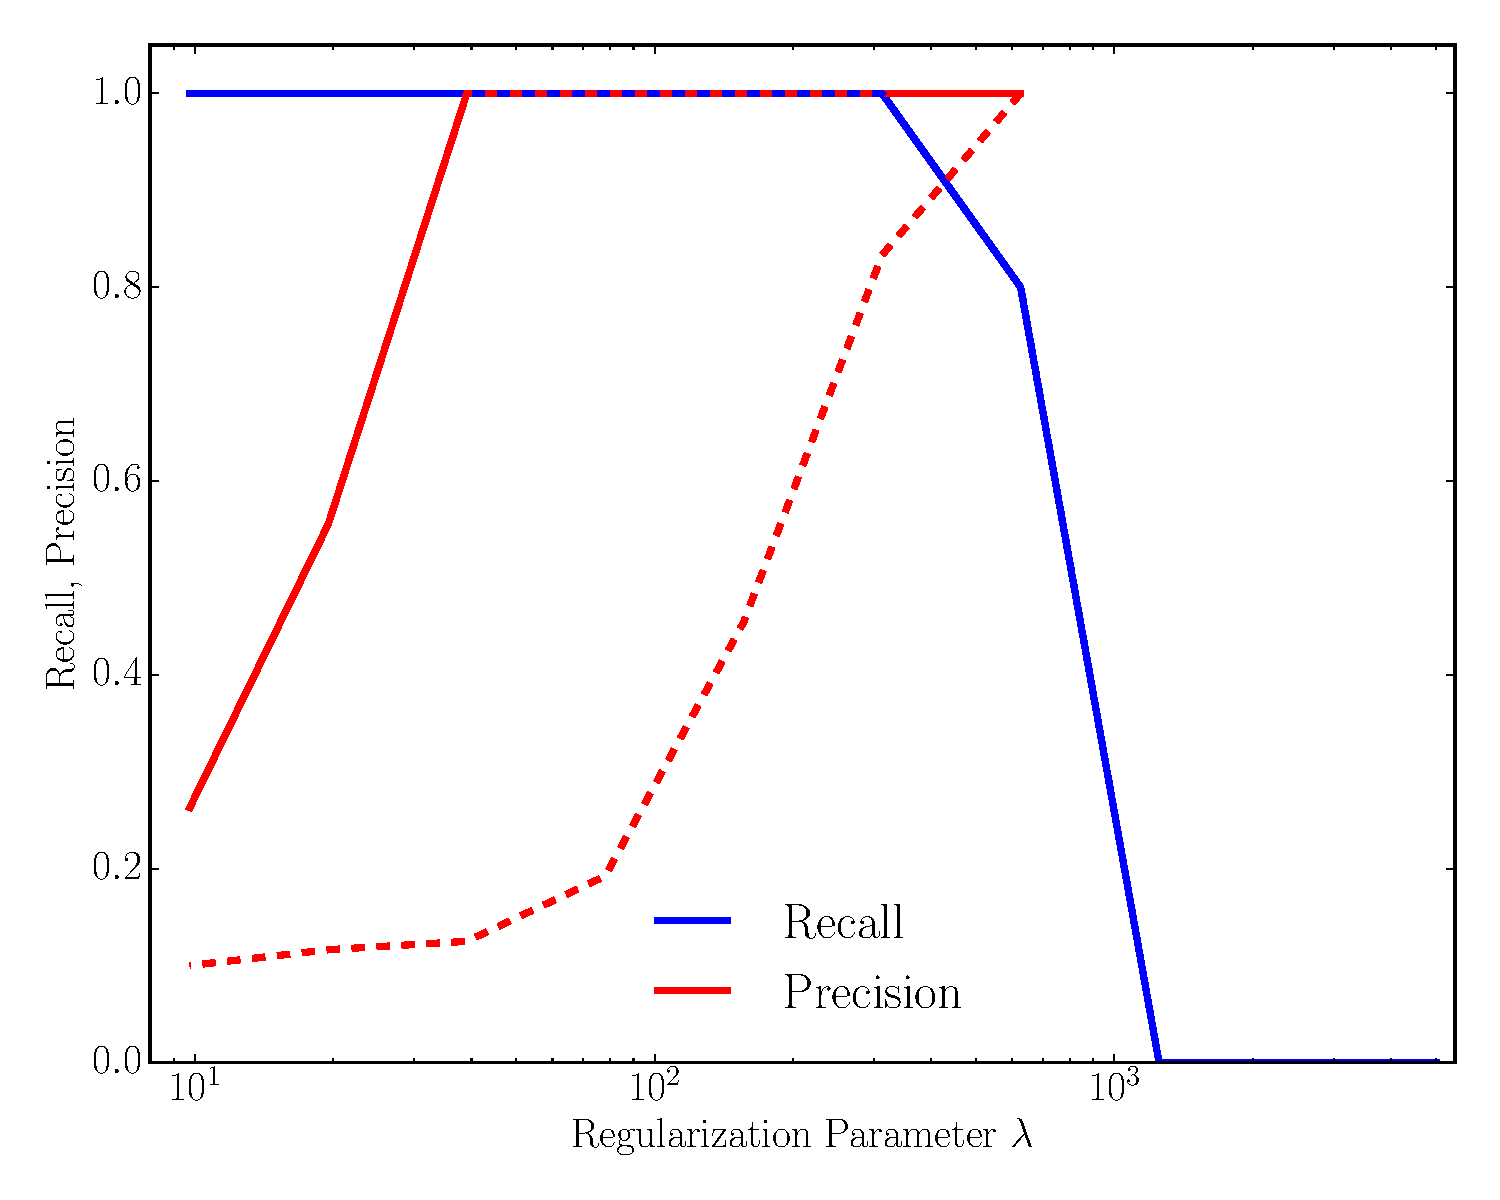
\includegraphics[width=\columnwidth]{synthetic_prec_rec.pdf}
    \caption{Precision (red curves) and recall (blue curves) as a function of the regularization coefficient $\lambda$ over a regularization path.  Solid curves represent data generated with $\sigma = 1$ while dashed curves represent noisy data generated assuming $\sigma = 10$.  For a given $\lambda$, the fitting the noisy $\sigma = 10$ data using the LASSO algorithm yields less precise answers but comparable recall relative to the $\sigma = 1$ data}
    \label{fig:synth_reg}
\end{figure}

For data generated with $\sigma = 1$ (solid curves in Fig.~\ref{fig:synth_reg}), a $\lambda \sim 10^3$ gives perfect precision and recall.  Larger $\lambda$s yield a larger regularization penalty which enforces a sparser solution, causing correct non-zero values to go to 0 resulting in worse recall and precision.  Smaller $\lambda$s have little effect on recall.  The LASSO algorithm tends towards ordinary least squares regression for smaller $\lambda$ and hence is still able to correctly determine the true non-zero values giving the observed perfect recall.  In this regime, however, the reduce penalty term also allows terms in $\hat{\omega}$ that should be 0 to become non-zero due to the regression algorithm overfitting the inherent noise in the data.  The additional non-zero terms arising from overfitting the noise drives the precision down as $\lambda$ decreases as the number of correct non-zeros in $\hat{\omega}$ stays the same while the total number of non-zero terms grows.

\subsection*{7.3.2}

I reran the same regularization analysis for the data generated with $\sigma = 10$ (dashed curves in Fig.~\ref{fig:synth_reg}) as I did for the $\sigma = 1$ data over the same $\lambda$ regularization path allowing for a direct comparison of the algorithm's performance for a given $\lambda$.  In general, I found that the recall was relatively unchanged between the two fits for all $\lambda$.  This makes sense since too large a $\lambda$ drives all $\hat{\omega}$ to 0 while smaller $\lambda$ allows for the linear regression to recover the correct non-zero values of $\omega_{true}$.  The precision for the fits on the data generated with $\sigma = 10$, however, was much worse than the fits over the $\sigma = 1$ data for almost all values of $\lambda$.  The enhanced noise in that synthetic dataset makes overfitting an issue and hence underscores the importance of regularization.  At larger $\lambda$, the precision is reasonable as the regularization penalty prevents the LASSO algorithm from overfitting and producing more incorrect non-zero terms in $\hat{\omega}$.  Smaller $\lambda$, however, yield a weaker regularization penalty and hence the algorithm overfits, producing many incorrect non-zero terms in $\hat{\omega}$ in giving poor precision.  

In order to achieve the optimal precision and recall for this noisy data, one should run a regularization path as before while monitoring recall.  Once recall has increased to 1, that $\lambda_{best}$ should be returned as the optimal regularization coefficient.  For $\lambda < \lambda_{best}$, the regularization penalty would be too low allowing noise to produce spurious features yielding incorrect non-zero terms in $\hat{\omega}$.  For the general case where $\omega_{true}$ is not known, one should bias towards larger $\lambda$ for noisy data to prevent overfitting.

Note: On this question, I collaborated with Matt Wilde, Serena Liu, and Janet Matsen.

\end{document}